\begin{figure*}[t!]
    \centering
    \begin{subfigure}[b]{0.2\linewidth}
        \centering
        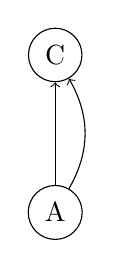
\begin{tikzpicture}[node distance=2cm]
                % First ANN
                \node[draw, circle] (A) at (0,0) {A};
                \node[draw, circle] (C) at (0,2) {C};
                
                \draw [->] (A) -- (C);
                \draw [->, bend right] (A) to (C);
            \end{tikzpicture}
            \caption{C=A}
            \label{ANNs1}
    \end{subfigure} \hfill
    \begin{subfigure}[b]{0.2\linewidth}
        \centering
       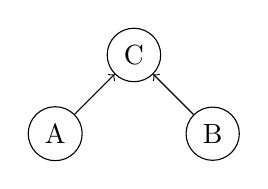
\begin{tikzpicture}[node distance=2cm]
            % Second ANN
            \node[draw, circle] (A) at (0, 0) {A}; 
            \node[draw, circle] (B) at (2, 0) {B}; 
            \node[draw, circle] (C) at (1, 1) {C}; 
            
            \draw [->] (A) -- (C);
            \draw [->] (B) -- (C);
        \end{tikzpicture}
        \caption{C = A $\land$ B}
        \label{ANNs2}
    \end{subfigure} \hfill
    \begin{subfigure}[b]{0.35\linewidth}
        \centering
        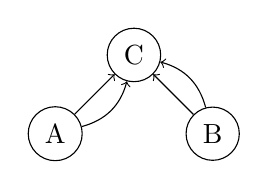
\begin{tikzpicture}[node distance=2cm]
            % Third ANN
            \node[draw, circle] (A) at (0, 0) {A};
            \node[draw, circle] (B) at (2, 0) {B};
            \node[draw, circle] (C) at (1, 1) {C};
            
            \draw [->] (A) -- (C);
            \draw [->, bend right] (A) to (C);
            \draw [->] (B) -- (C);
            \draw [->, bend right] (B) to (C);
        \end{tikzpicture}
        \caption{C = A $\lor$ B}
        \label{ANNs3}
    \end{subfigure} 
    \begin{subfigure}[b]{0.2\linewidth}
        \centering
        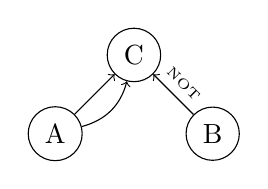
\begin{tikzpicture}[node distance=2cm]
            % Fourth ANN
            \node[draw, circle] (A) at (0, 0) {A};
            \node[draw, circle] (B) at (2, 0) {B};
            \node[draw, circle] (C) at (1, 1) {C};

            \draw [->] (A) -- (C);
            \draw [->, bend right] (A) to (C);
            \draw [->] (B) -- node[above, font=\tiny, sloped] {NOT} (C);
            
        \end{tikzpicture}
        \caption{C=A $\land \lnot$ B}
        \label{ANNs4}
    \end{subfigure}
    \caption{Artificial Neural Networks (ANNs) Performing Logical Computations - ANNs use multiple layers of neurons to perform logical computations.}
\end{figure*}
